%!TEX root = report.tex
This section presents the results of the two experiments discussed in \cref{s:experiment}.

\Crefrange{tab:results:1D:10:1000}{tab:results:1D:1000:10000} in \cref{a:results1D} present the results of the experiment with the one dimensional model.

The average energy, specific heat and average magnetization per spin for the different combinations of \numberOfSpins and \numberOfSamples can be found in \cref{fig:results:2D}. $d = 5, N_\textit{samples} = 1E+03$

\begin{figure}
	\centering
	\begin{subfigure}{\columnwidth}
		\centering
		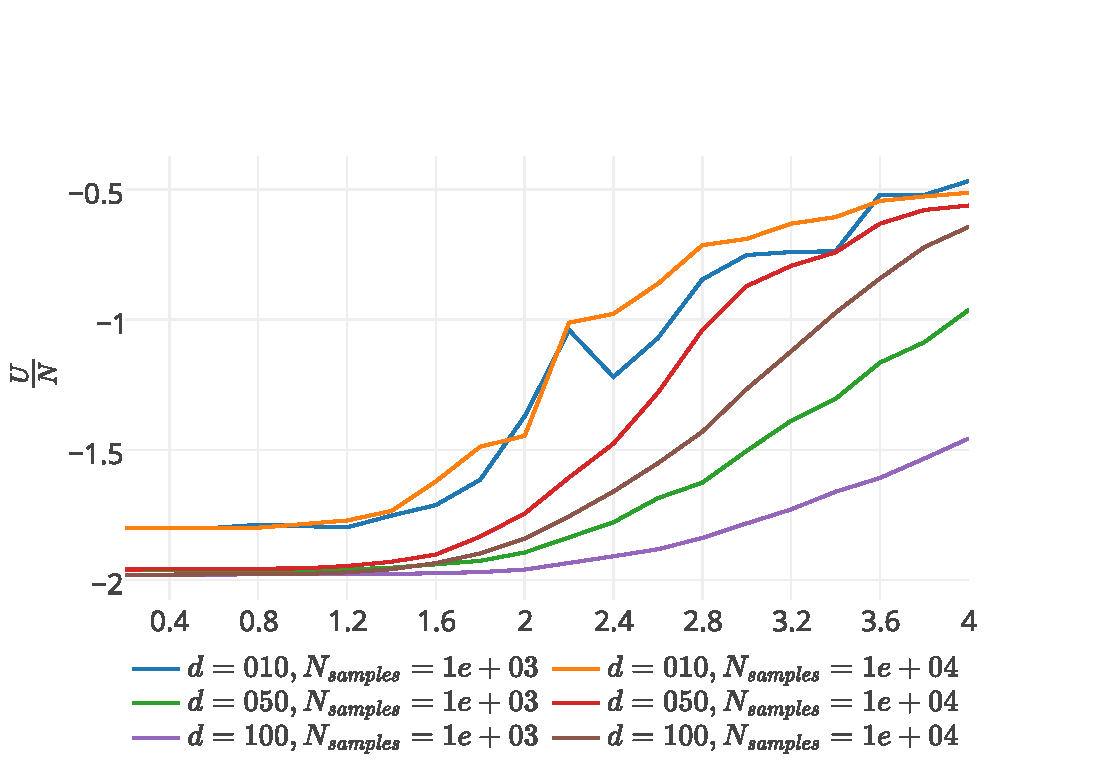
\includegraphics[width=\textwidth]{./img/2D/averageEnergy}
		\caption{Average energy per spin.}
		\label{fig:results:2D:averageEnergy}
	\end{subfigure}
	\begin{subfigure}{\columnwidth}
		\centering
		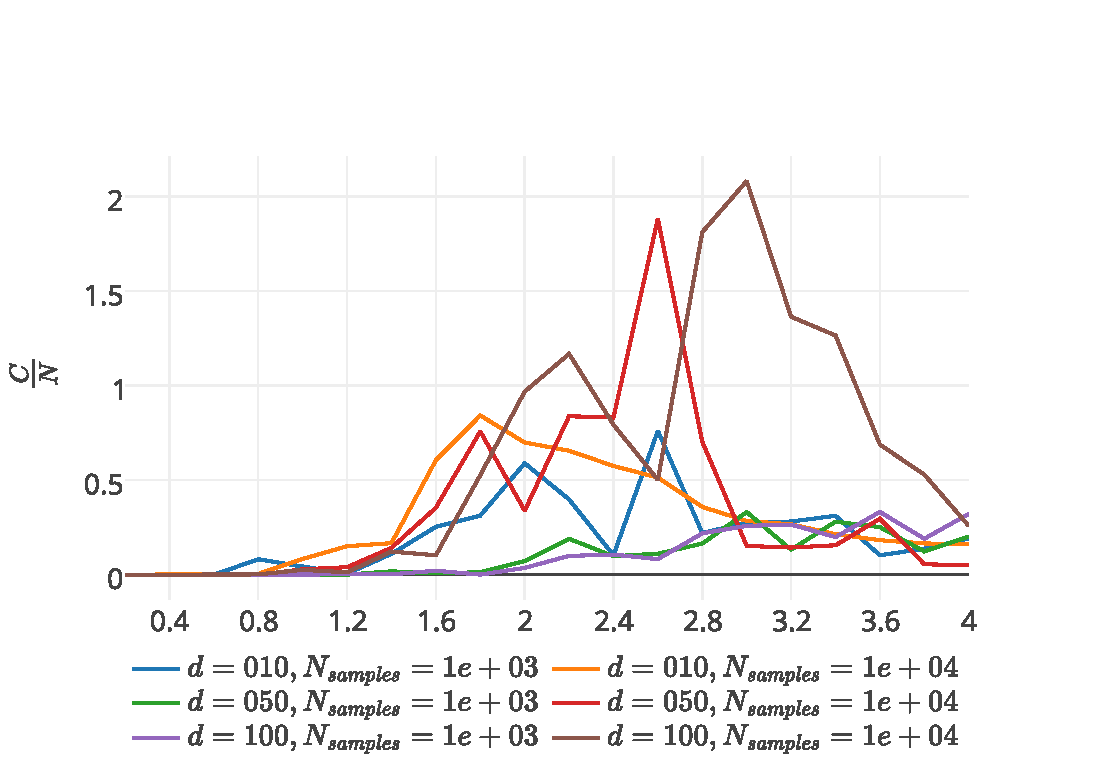
\includegraphics[width=\textwidth]{./img/2D/specificHeat}
		\caption{Average magnetization per spin.}
		\label{fig:results:2D:specificHeat}
	\end{subfigure}	
	\begin{subfigure}{\columnwidth}
		\centering
		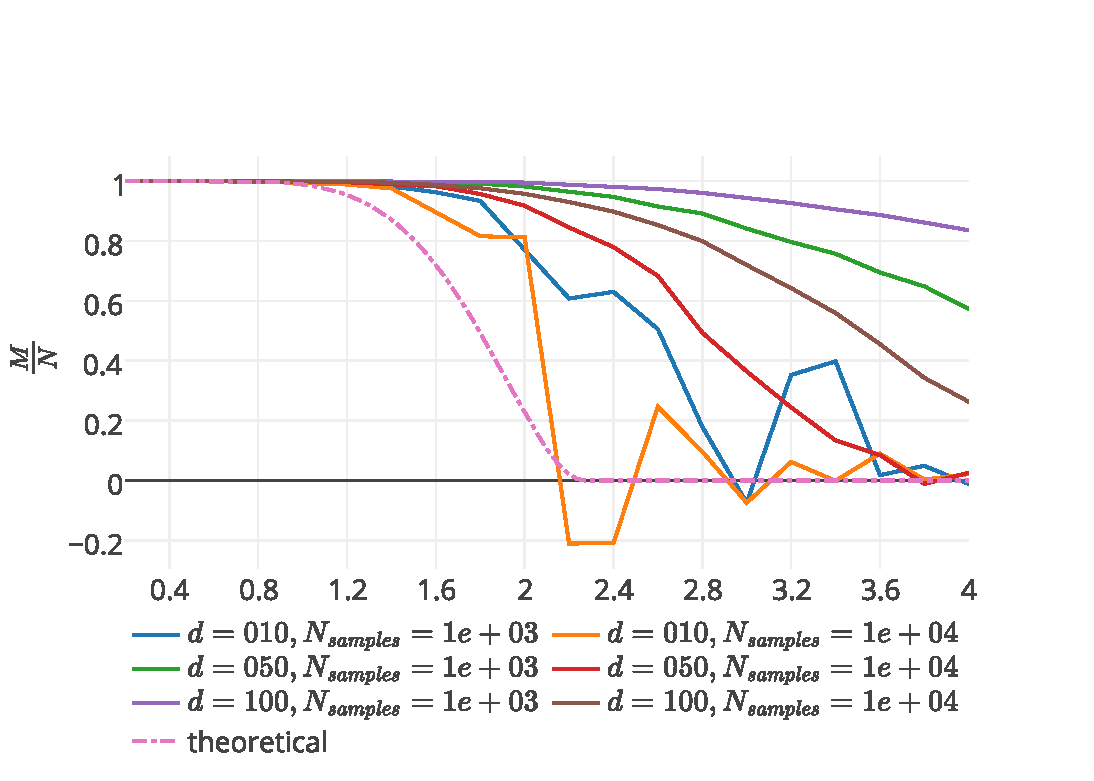
\includegraphics[width=\textwidth]{./img/2D/averageMagnetization}
		\caption{Average magnetization per spin.}
		\label{fig:results:2D:averageMagnetization}
	\end{subfigure}		
	\caption{The \subref{fig:results:2D:averageEnergy} average energy, \subref{fig:results:2D:specificHeat} specific heat and \subref{fig:results:2D:averageMagnetization} average magnetization per spin in a 2D Ising model with $\dimensionality = 10, 50, 100$ and $\numberOfSamples = 1000, 10000$.}
	\label{fig:results:2D}
\end{figure}